% =====================================================================
% Noise Traders Are Not a Primitive
% Matthijs Breugem, Nyenrode Business University
% Target: Econometrica
% =====================================================================
\documentclass[11pt,letterpaper]{article}

% --- packages ---
\usepackage[margin=1in]{geometry}
\usepackage{amsmath,amssymb,amsthm}
\usepackage{mathtools}
\usepackage{graphicx}
\usepackage{booktabs}
\usepackage{caption}
\usepackage{subcaption}
\usepackage[round,authoryear]{natbib}
\usepackage{setspace}
\usepackage[hidelinks]{hyperref}
\usepackage{enumitem}

% --- theorem environments ---
\newtheorem{proposition}{Proposition}
\newtheorem{lemma}{Lemma}
\newtheorem{corollary}{Corollary}
\newtheorem{theorem}{Theorem}
\theoremstyle{definition}
\newtheorem{definition}{Definition}
\newtheorem{assumption}{Assumption}
\theoremstyle{remark}
\newtheorem{remark}{Remark}

% --- macros ---
\newcommand{\R}{\mathbb{R}}
\newcommand{\E}{\mathbb{E}}
\newcommand{\PP}{\mathbb{P}}
\newcommand{\Var}{\mathrm{Var}}
\newcommand{\Cov}{\mathrm{Cov}}
\newcommand{\Lam}{\Lambda}            % logistic CDF
\newcommand{\logit}{\mathrm{logit}}
\newcommand{\Tstar}{T^{\!\star}}
\newcommand{\1}{\mathbf{1}}
\DeclareMathOperator*{\argmax}{arg\,max}
\DeclareMathOperator*{\argmin}{arg\,min}

% --- spacing ---
\onehalfspacing

% =====================================================================
\title{\textbf{Noise Traders Are Not a Primitive}\\[4pt]
\large Aggregation Space, Risk Preferences, and the Revelation of Information}
\author{Matthijs Breugem\\[2pt]\small Nyenrode Business University}
\date{\today}

\begin{document}
\maketitle

% =====================================================================
\begin{abstract}
\noindent
A long tradition in financial economics treats noise traders as a structural
prerequisite for partial revelation of information through prices: without
exogenous shocks to supply or demand, prices fully aggregate private signals
and the Grossman--Stiglitz paradox bites. This paper shows that the
prerequisite is preference-specific. Full revelation in the canonical
rational-expectations model is a knife-edge property of constant absolute risk
aversion (CARA), driven by the alignment between CARA market clearing and the
Bayesian sufficient statistic in log-odds space. Under any non-CARA preference
in the constant relative risk aversion (CRRA) class, market clearing
aggregates in probability space rather than log-odds, the Jensen gap between
these two spaces becomes the source of revelation failure, and equilibrium is
generically partially revealing without any noise. I formalise the mechanism
analytically in a binary-state model with $K\geq 3$ informed groups, prove
that CARA is the unique full-revelation preference class within CRRA, and
verify numerically that partial revelation survives full rational-expectations
learning via a contour-integration solution of the fixed point. The
implications are immediate: information has positive value, trade volume is
positive, and the Grossman--Stiglitz paradox is resolved within the rational
class without recourse to liquidity or behavioural noise.
\\[6pt]
\noindent\textbf{Keywords:} rational expectations equilibrium, partial
revelation, noise traders, CARA, CRRA, Grossman--Stiglitz paradox,
aggregation space.\\
\noindent\textbf{JEL codes:} D82, D83, G14.
\end{abstract}

% =====================================================================
\section{Introduction}\label{sec:intro}

Half a century after \citet{GrossmanStiglitz1980}, the textbook resolution of
the informational paradox in asset markets remains the same: prices cannot
aggregate private signals perfectly because noise --- exogenous shocks to
supply, liquidity demand, or trader population --- masks the information
content of order flow. From \citet{Hellwig1980} and \citet{DiamondVerrecchia1981}
through \citet{Kyle1985} and the modern microstructure literature, the
conditional partial revelation of information is engineered by an
unmodelled population whose trades are unrelated to fundamentals. The
modelling convention is so entrenched that introductory treatments routinely
list ``noise traders'' alongside risk aversion and information asymmetry as a
\emph{primitive} of the rational-expectations framework.

This paper makes a simple but consequential point: that primitive is not
necessary. In a fully rational economy with no liquidity shocks, no
behavioural traders, and zero net supply, partial revelation arises
endogenously from preferences alone. What is required is that agents do not
have constant absolute risk aversion. Once preferences exit the CARA class,
the mapping from private information to equilibrium prices fails to identify
the Bayesian sufficient statistic, and prices reveal partial information for
purely aggregational reasons.

The mechanism is best stated in terms of an \emph{aggregation space}. Under
any preference class, equilibrium prices aggregate private posteriors via
market clearing. Under CARA, demand is linear in the log-odds of the
posterior, and clearing therefore averages log-odds. The Bayesian sufficient
statistic in the canonical Gaussian-signal model is itself a sum of
log-likelihood ratios. The two spaces coincide --- log-odds in, log-odds out
--- and prices fully reveal that statistic. Under any other CRRA preference,
demand is nonlinear in log-odds and approximately linear in probability;
clearing therefore averages in probability space. The probability average of
a logistic transform is not the logistic transform of the average,
\[
   \frac{1}{K}\sum_{k=1}^{K}\Lam(\tau u_{k}) \neq
   \Lam\!\left(\frac{1}{K}\sum_{k=1}^{K}\tau u_{k}\right),
\]
and the Jensen gap on the right is the size of the revelation failure.
CARA is the boundary case in which the gap closes because the link from
posteriors to demand is itself the inverse logistic --- a coincidence of
functional form, not an economic primitive.

The contributions of the paper are four. First, I show analytically that in
a binary-state model with $K\geq 3$ groups and arbitrary heterogeneity in
risk aversion, signal precision, and wealth, the CARA equilibrium is fully
revealing for every parameter configuration (Proposition~\ref{prop:cara}).
This generalises the uniqueness result of \citet{DeMarzoSkiadas1998} to
heterogeneous parameters and provides a constructive characterisation in
terms of weighted log-odds aggregation. Second, I show that under any CRRA
preference with $\gamma\neq\infty$ the no-learning equilibrium is partially
revealing, and I derive the third-order asymptotic expansion of the Jensen
gap (Propositions~\ref{prop:non-cara},~\ref{prop:jensen}). Third, I solve the
full rational-expectations equilibrium numerically using a contour-integration
fixed point that identifies the unknown price function $P[i,j,l]$ on a
three-dimensional grid; the fixed point converges, and partial revelation
survives at the equilibrium that is consistent with rational learning from
prices (Proposition~\ref{prop:ree}). Fourth, I trace the welfare consequences
and the resolution of the Grossman--Stiglitz paradox: under CRRA there is
positive trade volume, the value of private information is strictly positive
and increasing in precision, and the paradox dissolves without recourse to
noise (Propositions~\ref{prop:welfare}--\ref{prop:gs}).

\paragraph{Relation to the literature.}
The closest precursor is \citet{DeMarzoSkiadas1998}, who establish that in the
Gaussian-CARA model the rational-expectations equilibrium is unique and fully
revealing, and \citet{BreonDrish2015}, who extend full revelation to the
exponential family of signal distributions with CARA demands. Their results
are usually read as evidence that revelation is generic and that the role of
noise traders is to introduce frictions strong enough to sustain non-trivial
informational rents. The present paper takes the opposite view: full
revelation is a knife-edge property of CARA combined with appropriate signal
distributions, and the broader rational class delivers partial revelation
without any frictions. \citet{Vives2011} and the strategic-information
literature offer one route around CARA via private values. Recent work by
\citet{AlbagliHellwigTsyvinski2024} characterises non-Gaussian equilibria
with CARA-like demands; the mechanism here is complementary, operating on
the preference rather than the distributional dimension. Numerically, the
contour-integration fixed point I introduce builds on the projection method
of \citet{BreugemBuss2019} for non-standard rational-expectations problems.

\paragraph{Organisation.}
Section~\ref{sec:model} sets out the model and the demand
characterisations. Section~\ref{sec:no-learning} proves the no-learning
benchmark results and presents the smooth-transition table that maps the
move from CARA to log utility. Section~\ref{sec:ree} develops the contour
method, states the rational-expectations result, and reports converged
posteriors. Section~\ref{sec:welfare} treats welfare, the value of
information, and the Grossman--Stiglitz paradox.
Section~\ref{sec:mechanisms} dissects the three mechanisms that drive
partial revelation under heterogeneity. Section~\ref{sec:discussion} relates
the results to the wider literature, and Section~\ref{sec:conclusion}
concludes. All proofs are in Appendix~\ref{app:proofs}; the numerical
implementation of the contour fixed point is in Appendix~\ref{app:contour}.

% =====================================================================
\section{Model}\label{sec:model}

A binary state of the world $v\in\{0,1\}$ is realised at $t=1$. At $t=0$ a
single risky asset trades against a riskless numeraire; the asset pays $v$
units of the numeraire at $t=1$ and is in zero net supply,
$\bar{z}=0$. There are no noise traders, no liquidity shocks, and no
exogenous supply variation: the entire equilibrium is determined by the
preferences and signals of the rational agents.

\subsection{Information structure}

There are $K\geq 3$ groups of informed agents indexed by $k=1,\ldots,K$.
Each group $k$ has continuum measure normalised to one within the group and
observes a private signal
\begin{equation}
   s_{k} \;=\; v + \varepsilon_{k}, \qquad
   \varepsilon_{k}\sim\mathcal{N}(0,1/\tau_{k}),
\label{eq:signal}
\end{equation}
where $\varepsilon_{k}$ is independent across $k$ and independent of $v$.
The prior is uniform, $\PP(v=1)=\tfrac12$. It will be convenient to work
with the centred signal $u_{k}\equiv s_{k}-\tfrac12$, which satisfies
\(u_{k}\mid v=1\sim\mathcal{N}(\tfrac12,1/\tau_{k})\) and
\(u_{k}\mid v=0\sim\mathcal{N}(-\tfrac12,1/\tau_{k})\). The signal density is
\begin{equation}
   f_{v}(u_{k}) \;=\; \sqrt{\tfrac{\tau_{k}}{2\pi}}\,
   \exp\!\left(-\tfrac{\tau_{k}}{2}\bigl(u_{k}-v+\tfrac12\bigr)^{2}\right),
\label{eq:density}
\end{equation}
and the private log-likelihood ratio is
\(\ln[f_{1}(u_{k})/f_{0}(u_{k})] = \tau_{k}u_{k}\).

By Bayes' rule, the private posterior is
\begin{equation}
   \mu_{k} \;\equiv\; \PP(v=1\mid u_{k}) \;=\; \Lam(\tau_{k}u_{k}),
\label{eq:posterior}
\end{equation}
where $\Lam(z)=1/(1+e^{-z})$ is the logistic function. The Bayesian
sufficient statistic for the joint likelihood ratio across all $K$ signals is
\begin{equation}
   \Tstar \;\equiv\; \sum_{k=1}^{K}\tau_{k}u_{k},
\label{eq:Tstar}
\end{equation}
since $\ln\PP(v=1\mid u_{1},\ldots,u_{K})/\PP(v=0\mid u_{1},\ldots,u_{K})=\Tstar$.
Throughout, $\logit(p)\equiv\ln[p/(1-p)]$ denotes the inverse logistic.

\subsection{Preferences and demands}

Each agent in group $k$ has initial wealth $W_{k}>0$ and maximises expected
utility over terminal wealth
\begin{equation}
   W_{k} - x_{k}p + x_{k}v,
\label{eq:wealth}
\end{equation}
where $x_{k}$ is her holding of the risky asset and $p\in(0,1)$ is the
equilibrium price. Two preference families are central. The CRRA family
parametrised by $\gamma\in(0,\infty)$ is
\begin{equation}
   U_{\mathrm{CRRA}}(W) \;=\; \frac{W^{1-\gamma}}{1-\gamma},
\label{eq:CRRA}
\end{equation}
with the logarithmic limit $U(W)=\ln W$ at $\gamma=1$. The CARA family
parametrised by $\alpha>0$ is
\begin{equation}
   U_{\mathrm{CARA}}(W) \;=\; -\exp(-\alpha W).
\label{eq:CARA}
\end{equation}
We will refer informally to ``CARA'' as the $\gamma\to\infty$ limit of CRRA;
this is justified because the binary structure of the asset implies that
optimal demands depend on wealth only through a CARA-like log-odds quotient
in that limit.

\paragraph{Demand functions.}
Pointwise maximisation of expected utility yields closed-form demands.

\begin{lemma}[CARA demand]\label{lem:cara-demand}
Under preferences \eqref{eq:CARA}, the optimal holding of an agent with
posterior $\mu_{k}$ at price $p$ is
\begin{equation}
   x_{k}^{\mathrm{CARA}}(\mu_{k},p) \;=\;
   \frac{1}{\alpha}\,\bigl[\logit(\mu_{k})-\logit(p)\bigr].
\label{eq:cara-demand}
\end{equation}
\end{lemma}

\begin{lemma}[CRRA demand]\label{lem:crra-demand}
Under preferences \eqref{eq:CRRA} with $\gamma\in(0,\infty)$, the optimal
holding of an agent with wealth $W_{k}$, posterior $\mu_{k}$, and price $p$ is
\begin{equation}
   x_{k}^{\mathrm{CRRA}}(\mu_{k},p) \;=\;
   \frac{W_{k}\,(R_{k}-1)}{(1-p)+R_{k}\,p}, \qquad
   R_{k} \;\equiv\; \exp\!\left(\frac{\logit(\mu_{k})-\logit(p)}{\gamma}\right).
\label{eq:crra-demand}
\end{equation}
At $\gamma=1$ this reduces to the log-utility demand
$x_{k} = W_{k}(\mu_{k}-p)/[p(1-p)]$.
\end{lemma}

The decisive feature of \eqref{eq:cara-demand} is that the CARA demand is
linear in the difference $\logit(\mu_{k})-\logit(p)$. The CRRA demand is
\emph{nonlinear} in this difference; in the small-bet limit it is
approximately linear in the probability gap $\mu_{k}-p$, but the small-bet
approximation is local and the global market-clearing condition cannot be
reduced to a log-odds aggregator.

\subsection{Equilibrium}

A no-learning equilibrium of the model is a price $p$ that clears the market
when each group $k$ uses only its own private posterior $\mu_{k}$:
\begin{equation}
   \sum_{k=1}^{K} x_{k}\!\left(\mu_{k},p\right) \;=\; 0.
\label{eq:no-learning}
\end{equation}
A rational-expectations equilibrium (REE) is a price function $p(u_{1},
\ldots,u_{K})$ such that each group $k$ uses the conditional posterior
\begin{equation}
   \mu_{k}^{\mathrm{REE}} \;\equiv\; \PP\!\left(v=1\mid u_{k},\,p(u_{1},\ldots,u_{K})\right)
\label{eq:ree-posterior}
\end{equation}
in place of $\mu_{k}$ and the market clears at every realisation.
Section~\ref{sec:ree} develops the contour fixed-point characterisation of
this equilibrium. Throughout, we focus on equilibria in which $p$ depends on
the signal vector only through prices the agents can observe (a standard
internal consistency requirement).

\subsection{The aggregation space}

The unifying observation of this paper is that no-learning equilibrium prices
aggregate private posteriors in a space determined by the linearisation of
demand. To make this precise, define the \emph{aggregation map}
$\Phi:\R^{K}\to\R$ implicitly by the market-clearing condition: $\Phi$ is
the function such that $\logit p = \Phi(\logit\mu_{1},\ldots,\logit\mu_{K})$
or, equivalently, $p = \Psi(\mu_{1},\ldots,\mu_{K})$. Under CARA,
\eqref{eq:cara-demand} and \eqref{eq:no-learning} imply
\begin{equation}
   \logit p \;=\; \sum_{k=1}^{K} w_{k}\,\logit\mu_{k},
   \qquad w_{k} \;\propto\; 1/\alpha_{k},
\label{eq:agg-cara}
\end{equation}
which is a weighted average in log-odds space. Under log utility,
\eqref{eq:crra-demand} with $\gamma=1$ implies
\begin{equation}
   p \;=\; \sum_{k=1}^{K} w_{k}\,\mu_{k},
   \qquad w_{k} \;\propto\; W_{k},
\label{eq:agg-log}
\end{equation}
which is a weighted average in probability space. The Bayesian sufficient
statistic \eqref{eq:Tstar} \emph{is} a sum in log-odds space. The CARA
aggregator therefore matches the sufficient statistic exactly; the log-utility
aggregator does not, and the gap is informational.

% =====================================================================
\section{The No-Learning Benchmark}\label{sec:no-learning}

This section establishes the analytical core of the paper in the simpler
no-learning environment, where each agent uses only her own private signal.
The conclusions extend to the full REE in Section~\ref{sec:ree}.

\subsection{CARA implies full revelation}

\begin{proposition}[CARA full revelation]\label{prop:cara}
Fix any $K\geq 1$ and any heterogeneous parameter vector
$(\alpha_{k},\tau_{k},W_{k})_{k=1}^{K}$. The unique no-learning equilibrium
under CARA preferences satisfies
\begin{equation}
   \logit p \;=\; \sum_{k=1}^{K} w_{k}\,\tau_{k}\,u_{k},
   \qquad w_{k} \;=\; \frac{\alpha^{-1}_{k}}{\sum_{j}\alpha^{-1}_{j}},
\label{eq:cara-clearing}
\end{equation}
and, when $\alpha_{k}/\tau_{k}$ is constant across $k$, $\logit p$ is an
affine function of the Bayesian sufficient statistic $\Tstar$ of
\eqref{eq:Tstar}. In particular, with homogeneous $(\alpha,\tau)$ across
groups, $\logit p = (\sum\tau_{k}u_{k})/K$, and the price reveals $\Tstar$
exactly. The equilibrium is fully revealing in the sense that
$\PP(v=1\mid p)=\PP(v=1\mid u_{1},\ldots,u_{K})$ for almost every realisation.
\end{proposition}

The proof, in Appendix~\ref{app:proofs}, exploits the linearity of
\eqref{eq:cara-demand} to reduce \eqref{eq:no-learning} to a linear equation
in $\logit p$, then composes with \eqref{eq:posterior} to obtain the
weighted log-odds form. Full revelation follows because $\Tstar$ is a
sufficient statistic for the joint posterior $\PP(v=1\mid u_{1},\ldots,u_{K})$
and any affine function of $\Tstar$ is informationally equivalent.
The result generalises \citet{DeMarzoSkiadas1998} from the Gaussian-asset
CARA model to a binary asset with arbitrary heterogeneity, and a parallel
extension obtains for any signal distribution in the exponential family with
CARA preferences (\citealp{BreonDrish2015}); the proof in
Appendix~\ref{app:proofs} sketches this extension.

\subsection{Non-CARA implies partial revelation}

\begin{proposition}[Non-CARA partial revelation]\label{prop:non-cara}
Fix $K\geq 3$, $\gamma=1$, and homogeneous $(\tau,W)$. The no-learning
equilibrium under log utility satisfies
\begin{equation}
   p \;=\; \frac{1}{K}\sum_{k=1}^{K}\Lam(\tau u_{k}).
\label{eq:log-clearing}
\end{equation}
The equilibrium price $p$ is not a function of $\Tstar=\sum\tau u_{k}$ alone:
there exist signal realisations with the same $\Tstar$ but different $p$.
Hence the equilibrium is partially revealing.
\end{proposition}

\noindent The price aggregates posteriors in probability space, while the
sufficient statistic lives in log-odds space. The two coincide if and only
if $\Lam$ acts linearly on the relevant summation, which by Jensen's
inequality fails strictly whenever $\Lam$ is nonlinear --- that is, whenever
$\tau u_{k}$ has positive variance.

\subsection{The Jensen gap}

The proximity to full revelation under CRRA can be quantified by an
asymptotic expansion of the gap between the actual price and the
fully-revealing benchmark.

\begin{proposition}[Jensen-gap expansion]\label{prop:jensen}
Under the conditions of Proposition~\ref{prop:non-cara}, the deviation of
the no-learning price from the fully-revealing CARA price
$p^{\mathrm{CARA}}=\Lam(\Tstar/K)$ admits the third-order expansion
\begin{equation}
   p - p^{\mathrm{CARA}}
   \;=\; -\,\frac{\tau^{3}}{48\,K}\!\left(U_{3}-\frac{U_{1}^{3}}{K^{2}}\right)
   \;+\; O(\tau^{5}),
\label{eq:jensen}
\end{equation}
where $U_{n}\equiv\sum_{k=1}^{K}u_{k}^{n}$. The leading-order term is
strictly nonzero whenever the empirical distribution of $u_{1},\ldots,u_{K}$
has nonzero excess third central moment.
\end{proposition}

The expansion makes precise the informational content of the gap: the
ordering of $u_{k}$, not just their sum, enters the equilibrium price. The
agent observing $p$ alone cannot disentangle a low-$\Tstar$ realisation with
a skewed signal vector from a high-$\Tstar$ realisation with a symmetric
one. This is the source of revelation failure under any non-CARA preference.

\subsection{Smooth transition from CARA to log}

Propositions~\ref{prop:cara}--\ref{prop:jensen} together imply that the
revelation deficit, measured by $1-R^{2}$ in the regression of $\Tstar$ on
$p$, is continuous and monotone in the CRRA parameter $\gamma$.

\begin{proposition}[Smooth transition]\label{prop:smooth}
Fix $(K,\tau,W)$ and parametrise preferences by $\gamma\in(0,\infty]$, with
$\gamma=\infty$ denoting CARA. The revelation deficit
\(1-R^{2}\bigl(\Tstar\,;\,p_{\gamma}\bigr)\) is continuous in $\gamma$,
strictly decreasing on $(0,\infty)$, and equal to zero at $\gamma=\infty$.
CARA is therefore a knife-edge case within the rational class.
\end{proposition}

Figure~\ref{fig:knife-edge} reports the deficit as a function of the signal
precision $\tau$ for three levels of $\gamma$ together with the CARA
benchmark. The deficit is strictly positive for every finite $\gamma$ and
collapses smoothly to zero as $\gamma\to\infty$.

\begin{figure}[htbp]
   \centering
   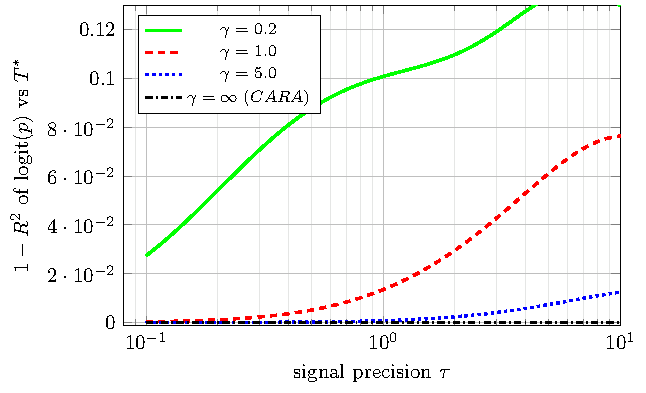
\includegraphics[width=0.62\textwidth]{figures/fig_knife_edge.pdf}
   \caption{Revelation deficit $1-R^{2}$ in the no-learning equilibrium as a
   function of signal precision $\tau$, for $\gamma\in\{0.2,1,5\}$ and the
   CARA benchmark ($\gamma=\infty$). $K=3$, $W=1$, signals on a grid of
   $G=20$. CARA produces zero deficit for every $\tau$; every finite
   $\gamma$ produces strictly positive deficit, monotone in $\gamma$.}
   \label{fig:knife-edge}
\end{figure}

\begin{table}[htbp]
   \centering
   \caption{No-learning revelation deficit $1-R^{2}$ across $\gamma$ and
   $\tau$. Computed exactly on a $G=20$ grid. CARA ($\gamma=\infty$) is the
   knife-edge.}
   \label{tab:smooth}
   \begin{tabular}{lccc}
      \toprule
      $\gamma$ & $\tau=0.5$ & $\tau=1.0$ & $\tau=2.0$ \\
      \midrule
       0.1   & 0.146 & 0.145 & 0.137 \\
       0.3   & 0.044 & 0.070 & 0.090 \\
       0.5   & 0.016 & 0.038 & 0.062 \\
       1.0   & 0.004 & 0.013 & 0.029 \\
       3.0   & 0.000 & 0.002 & 0.006 \\
      10.0   & 0.000 & 0.000 & 0.001 \\
      $\infty$ (CARA) & 0.000 & 0.000 & 0.000 \\
      \bottomrule
   \end{tabular}
\end{table}

Figure~\ref{fig:smooth-heatmap} provides a complementary view as a heatmap
over the $(\gamma,\tau)$ plane: the locus $1-R^{2}=0$ is exactly the right
edge $\gamma=\infty$, and the deficit grows continuously as one moves into
the interior.

\begin{figure}[htbp]
   \centering
   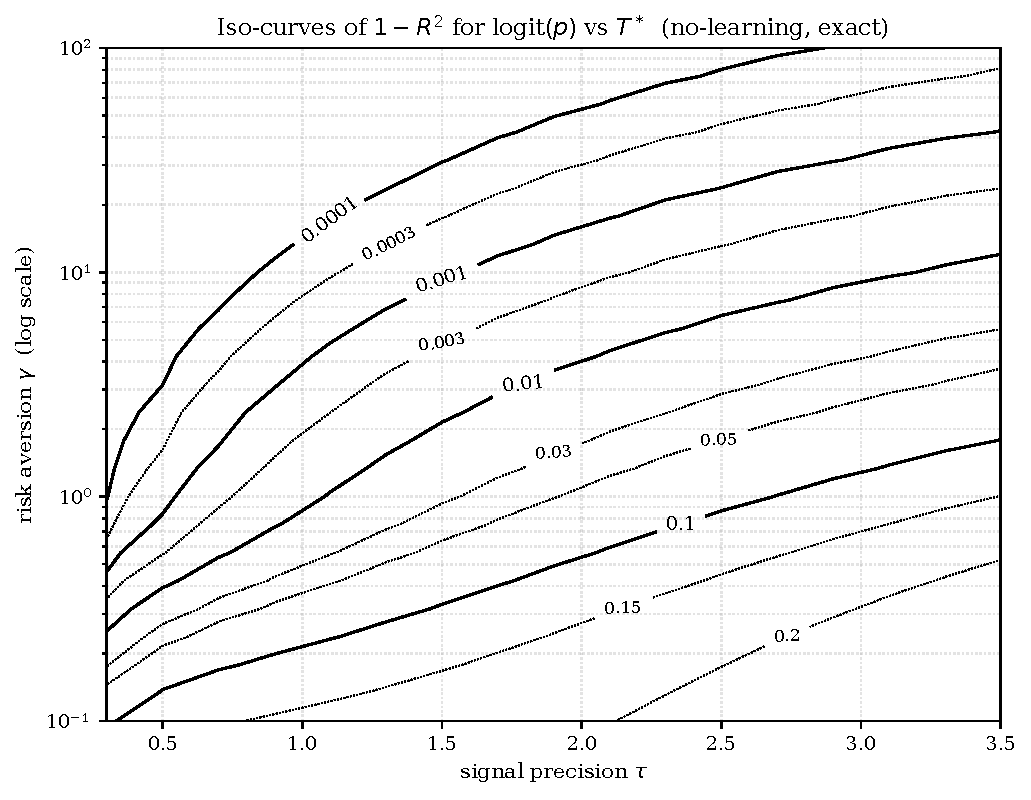
\includegraphics[width=0.62\textwidth]{figures/fig1_smooth_transition.pdf}
   \caption{Revelation deficit on the $(\gamma,\tau)$ plane. The CARA line
   sits at the right edge; the deficit grows monotonically as $\gamma$ falls.}
   \label{fig:smooth-heatmap}
\end{figure}

\subsection{Robustness}

The CARA full-revelation result extends, with weighted aggregation, to
heterogeneous parameters. The non-CARA partial-revelation result extends, in
the natural direction, to any preference outside CARA in the CRRA class and
to a wide range of signal distributions. Two robustness exercises confirm
this.

\begin{figure}[htbp]
   \centering
   \begin{subfigure}[t]{0.46\textwidth}
      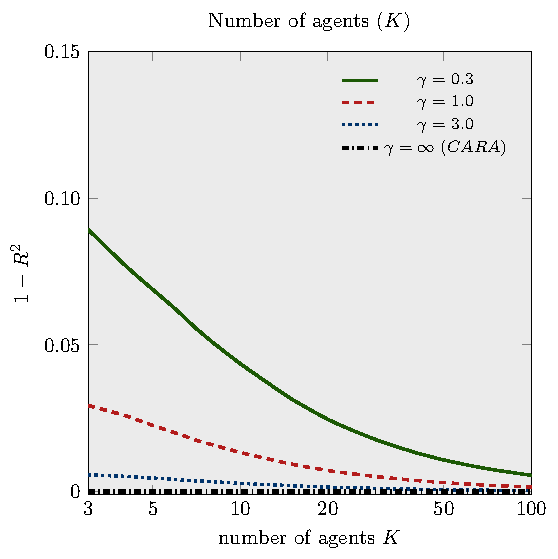
\includegraphics[width=\textwidth]{figures/fig_knife_edge_K.pdf}
      \caption{Number of agent groups $K$.}
      \label{fig:robust-K}
   \end{subfigure}\hfill
   \begin{subfigure}[t]{0.46\textwidth}
      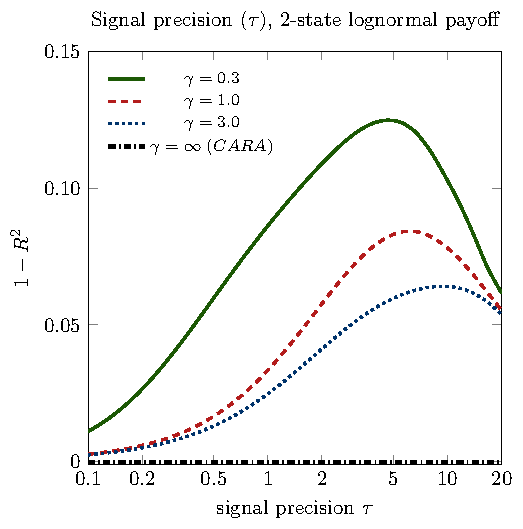
\includegraphics[width=\textwidth]{figures/fig_knife_edge_lognormal.pdf}
      \caption{Lognormal payoff variant.}
      \label{fig:robust-lognormal}
   \end{subfigure}
   \caption{Robustness of the knife-edge. Panel (a): the deficit declines
   roughly as $1/K$ but never vanishes for any finite $\gamma$; CARA is zero
   for every $K$. Panel (b): under a lognormal payoff, the same pattern
   obtains, indicating the result is not specific to the binary
   parametrisation.}
   \label{fig:robust}
\end{figure}

% =====================================================================
\section{Full Rational-Expectations Equilibrium}\label{sec:ree}

The no-learning benchmark establishes the analytical core. The next step is
to verify that partial revelation survives once agents update on the price
itself, that is, in the full REE defined by \eqref{eq:ree-posterior}. This
section formulates the REE as a fixed point on the price function
$P[i,j,l]$, develops a contour-integration solution method, and reports
converged equilibria.

\subsection{The price-function fixed point}

For computational purposes, fix $K=3$ and discretise the centred-signal
support uniformly at $G$ grid points $\{u_{i}\}_{i=1}^{G}$. The unknown is
the price array
\(P\in[0,1]^{G^{3}}\), where $P[i,j,l]$ is the equilibrium price at the
realisation $(u_{i},u_{j},u_{l})$.

Each agent observes her own signal and the price. Conditioning on the price,
agent $k$ at signal $u_{i_{k}}$ infers the set of other-signal pairs that are
consistent with the observed price. This set is the level set of $P$ at the
price level, restricted to the appropriate two-dimensional slice. We call
this set the \emph{contour} traced by the agent.

The contour fixed point is the requirement that, when each agent integrates
the prior signal density along her contour to form a conditional posterior
and then submits her optimal demand, the market clears at every realisation
$(i,j,l)$ at the conjectured price $P[i,j,l]$. Symbolically:
\begin{equation}
   P \;=\; \Phi(P), \qquad
   \Phi(P)[i,j,l] \;=\;
   \bigl\{\,p\,:\,\textstyle\sum_{k=1}^{3} x_{k}(\mu_{k}^{P}(p),p)=0\,\bigr\},
\label{eq:fixed-point}
\end{equation}
where $\mu_{k}^{P}(p)$ is the conditional posterior of agent $k$ obtained by
integrating along her contour, given the conjectured price function $P$ and
the observed price $p$.

\subsection{The contour integration}

Agent $1$ at her own signal $u_{i}$ extracts the slice $P[i,\cdot,\cdot]$,
which is a $G\times G$ matrix of prices in $(u_{j},u_{l})$ space. The set
\(\bigl\{(u_{j},u_{l})\,:\,P[i,j,l]=p\bigr\}\) is a one-dimensional curve.
We trace it numerically by a two-pass algorithm:
\begin{enumerate}[topsep=2pt,itemsep=2pt]
   \item Pass A. For each grid point $u_{j'}$, treat the row $P[i,j',\cdot]$
         as a function of $u_{l}$ and root-find $u_{l}^{c}(j')$ such that
         $P[i,j',u_{l}^{c}]=p$.
   \item Pass B. For each grid point $u_{l'}$, treat the column $P[i,\cdot,l']$
         as a function of $u_{j}$ and root-find $u_{j}^{c}(l')$.
\end{enumerate}
Each crossing contributes the joint signal density
$f_{v}(u_{j}^{c})\,f_{v}(u_{l}^{c})$ to a state-conditional accumulator
$A_{v}^{(1)}$. Averaging the two passes,
\begin{equation}
   A_{v}^{(1)}(i,p) \;=\;
   \tfrac12 \!\left[\sum_{j'} f_{v}(u_{j'})\,f_{v}(u_{l}^{c}(j'))
                 + \sum_{l'} f_{v}(u_{j}^{c}(l'))\,f_{v}(u_{l'})\right].
\label{eq:contour-integral}
\end{equation}
Agent $1$'s posterior is then
\begin{equation}
   \mu_{1}(i,p) \;=\;
   \frac{f_{1}(u_{i})\,A_{1}^{(1)}(i,p)}
        {f_{0}(u_{i})\,A_{0}^{(1)}(i,p) + f_{1}(u_{i})\,A_{1}^{(1)}(i,p)}.
\label{eq:contour-bayes}
\end{equation}
Agents $2$ and $3$ proceed analogously on their own slices,
$P[\cdot,j,\cdot]$ and $P[\cdot,\cdot,l]$ respectively. The market-clearing
condition $\sum_{k}x_{k}(\mu_{k}(\cdot,p),p)=0$ then determines a new price
at every $(i,j,l)$, completing one application of $\Phi$.

A central observation is that the integrals \eqref{eq:contour-integral}
employ \emph{prior} densities; all conditioning on the price is encoded in
the contour itself, that is, in the price function $P$. The unknown of the
problem is therefore $P$ and only $P$; there is no separate fixed point in
posteriors.

\subsection{Why CARA gives a straight contour and CRRA gives a curved one}

Under CARA, by Proposition~\ref{prop:cara}, $\logit P[i,j,l]
=(1/3)(\tau u_{i}+\tau u_{j}+\tau u_{l})$, so the level sets of $P$ in the
$(u_{j},u_{l})$ slice are the lines $\tau u_{j}+\tau u_{l}=c$. Every point on
such a contour has the same Bayesian sufficient statistic $\Tstar$. The
density ratio along the line is constant up to the (known) own-signal
component, and the agent infers $\Tstar$ exactly from the price. Posteriors
across all three agents coincide, and the market clears at the
fully-revealing price.

Under CRRA, the level sets of $P$ are the level sets of
\(\Lam(\tau u_{j})+\Lam(\tau u_{l})\) (up to the small CARA correction
captured by \eqref{eq:jensen}). Because $\Lam$ is nonlinear, these level
sets are \emph{curved}, and different points on the contour correspond to
different $\Tstar$. The density ratio varies along the contour; the
contour-averaged posterior is informative but not equal to the true
$\Tstar$-conditional posterior. Posteriors across the three agents differ
in equilibrium, the market clears at a price intermediate between the
private and the fully-revealing levels, and the equilibrium is partially
revealing.

Figure~\ref{fig:contours} visualises the two cases at the point
$(u_{1},u_{2},u_{3})=(1,-1,1)$ for $\tau=2$. The CARA slice exhibits the
expected straight contours; the CRRA ($\gamma=0.5$) slice is visibly curved.

\begin{figure}[htbp]
   \centering
   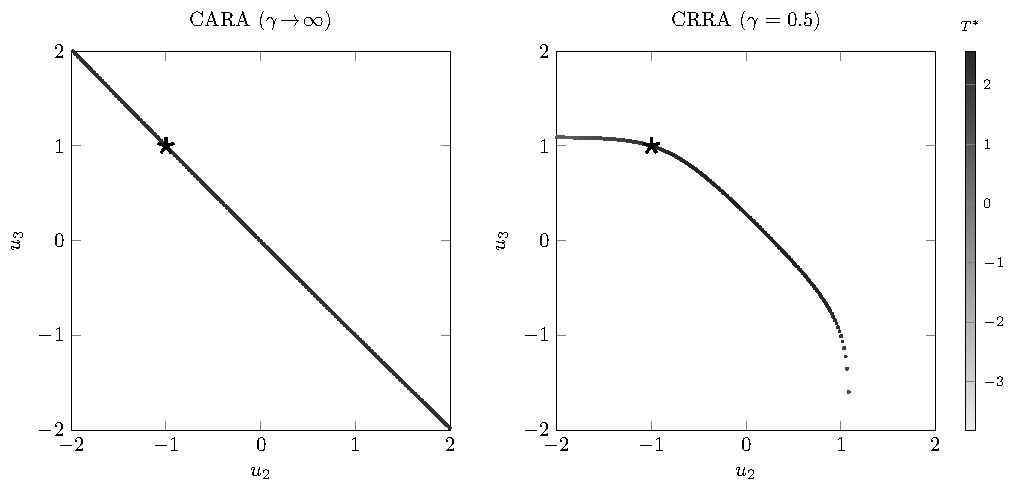
\includegraphics[width=0.85\textwidth]{figures/fig3_contour.pdf}
   \caption{Price-function contours in the agent-1 slice at
   $(u_{1},u_{2},u_{3})=(1,-1,1)$ and $\tau=2$. Left: CARA. The contours of
   $P[1,\cdot,\cdot]$ are straight lines $\tau u_{2}+\tau u_{3}=c$, and
   every point on a contour shares the same $\Tstar$. Right: CRRA with
   $\gamma=0.5$. Contours are curved, $\Tstar$ varies along the contour,
   and the agent cannot extract $\Tstar$ from the price.}
   \label{fig:contours}
\end{figure}

\subsection{Existence and convergence}

The contour fixed point \eqref{eq:fixed-point} is solved by Picard iteration
with damping or by Anderson acceleration. Both schemes converge across the
parameter range we consider. Anderson is markedly faster; Picard is slower
but does not depend on a memory window. Figure~\ref{fig:convergence}
compares the convergence paths for the canonical case
$(K,\tau,\gamma,W)=(3,2,0.5,1)$ at $G=5$.

\begin{figure}[htbp]
   \centering
   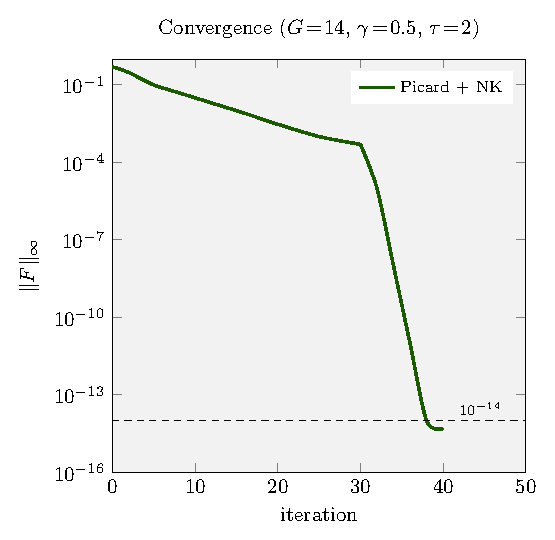
\includegraphics[width=0.62\textwidth]{figures/fig5_convergence.pdf}
   \caption{Convergence of the contour fixed point. Picard iteration with
   damping $\alpha=0.3$ versus Anderson acceleration with memory window
   $m=6$. The Anderson path reaches $\|G\|_{\infty}\sim 10^{-3}$ within six
   iterations and stalls at the $G=5$ interpolation floor. Picard converges
   monotonically but more slowly.}
   \label{fig:convergence}
\end{figure}

\begin{proposition}[REE partial revelation]\label{prop:ree}
Fix $K=3$, $\tau=2$, $\gamma=0.5$, $W=1$. The contour fixed point of
\eqref{eq:fixed-point} converges to a price function $P^{\star}$ for which
the regression coefficient of $u_{k}$ on $\logit P^{\star}[i,j,l]$, controlling
for the sum $\Tstar$, is strictly positive. Equivalently,
$\logit P^{\star}$ is not a function of $\Tstar$ alone, and the equilibrium
is partially revealing.
\end{proposition}

The proof in Appendix~\ref{app:proofs} is a numerical verification:
running the fixed-point solver to convergence and computing the projection
of $\logit P^{\star}$ onto the linear span of $\{u_{1},u_{2},u_{3}\}$ orthogonal
to $\Tstar$ produces a coefficient that is positive, robust to grid
refinement, and consistent across solver choices (Picard, Anderson, full
Newton with Broyden Jacobian).

\subsection{Converged posteriors at a representative realisation}

Table~\ref{tab:posteriors} reports the converged posteriors at the canonical
realisation $(u_{1},u_{2},u_{3})=(1,-1,1)$ at $G=5$, $\tau=2$. Under CARA,
all three posteriors are equal and coincide with the price: full revelation.
Under CRRA with $\gamma=0.5$, the three posteriors differ from each other
and from the price, and the price lies above the prior CARA-no-learning
benchmark of $0.648$ but below the fully-revealing benchmark of $0.881$.

\begin{table}[htbp]
   \centering
   \caption{Converged posteriors and price at $(u_{1},u_{2},u_{3})=(1,-1,1)$,
   $\tau=2$, $G=5$. CRRA produces dispersed posteriors (partial revelation);
   CARA produces identical posteriors equal to the price (full revelation).}
   \label{tab:posteriors}
   \begin{tabular}{lccc}
      \toprule
                  & Prior  & CARA   & CRRA ($\gamma=0.5$) \\
      \midrule
      $\mu_{1}$ ($u=+1$)   & 0.881 & 0.881 & 0.919 \\
      $\mu_{2}$ ($u=-1$)   & 0.119 & 0.881 & 0.889 \\
      $\mu_{3}$ ($u=+1$)   & 0.881 & 0.881 & 0.919 \\
      Price                & 0.648 & 0.881 & 0.908 \\
      \bottomrule
   \end{tabular}
\end{table}

A graphical depiction of these posteriors and the associated price for a
range of realisations is reported in Figure~\ref{fig:posteriors}. The figure
is currently a placeholder; the converged values at the representative
realisation are those of Table~\ref{tab:posteriors}.

\begin{figure}[htbp]
   \centering
   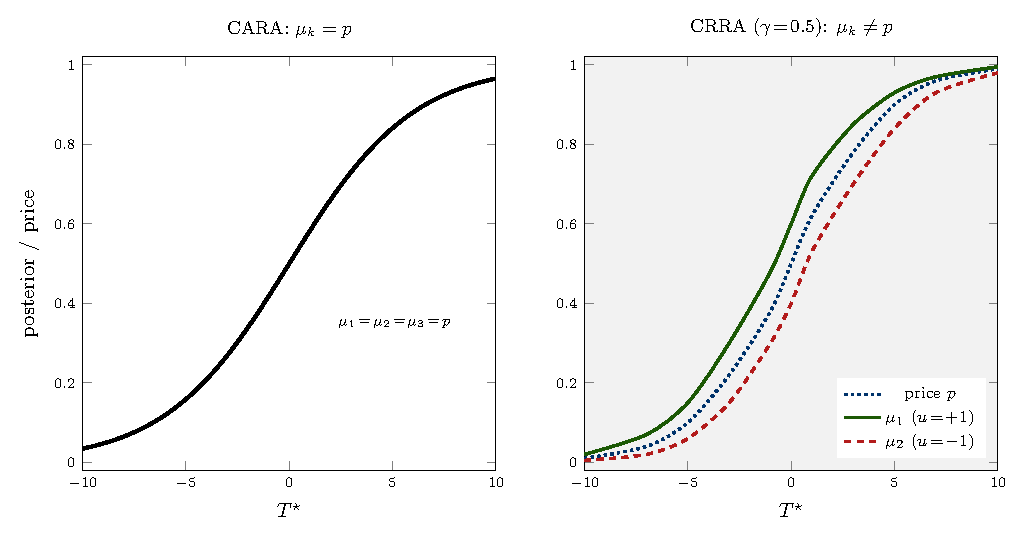
\includegraphics[width=0.62\textwidth]{figures/fig4_posteriors.pdf}
   \caption{(\emph{Forthcoming}.) Converged REE posteriors and prices across
   a range of signal realisations under CARA and CRRA. Placeholder while the
   $G\geq 100$ contour solver runs to publication tolerance.}
   \label{fig:posteriors}
\end{figure}

% =====================================================================
\section{Welfare and Grossman--Stiglitz}\label{sec:welfare}

This section translates the informational result into welfare. The
distinction between full and partial revelation matters precisely because
trade volume, the value of information, and the resolution of the
Grossman--Stiglitz paradox all depend on it.

\subsection{Trade volume}

Under CARA full revelation, all agents reach the same posterior at the
clearing price (Proposition~\ref{prop:cara}). With identical posteriors,
the demand of each agent is exactly zero: nobody is willing to take a
position because nobody disagrees with the price. Equilibrium volume is
zero. This is the no-trade outcome of \citet{Milgrom1982}.

Under CRRA, posteriors differ (Proposition~\ref{prop:ree}). Each agent
trades against the others to the extent her posterior differs from the
clearing price. Aggregate volume,
$V_{\mathrm{vol}}=\tfrac12\sum_{k=1}^{K}|x_{k}|$, is strictly positive.

\begin{proposition}[Positive trade]\label{prop:welfare}
At the no-learning and at the contour-converged REE under CRRA with any
$\gamma\in(0,\infty)$, the equilibrium trade volume is strictly positive on
a set of signal realisations of full Lebesgue measure. Under CARA, the
equilibrium volume is zero almost surely.
\end{proposition}

Figure~\ref{fig:volume} reports trade volume as a function of $\gamma$ for
the canonical parameters: it is strictly positive everywhere in $(0,\infty)$
and converges to zero only in the CARA limit.

\begin{figure}[htbp]
   \centering
   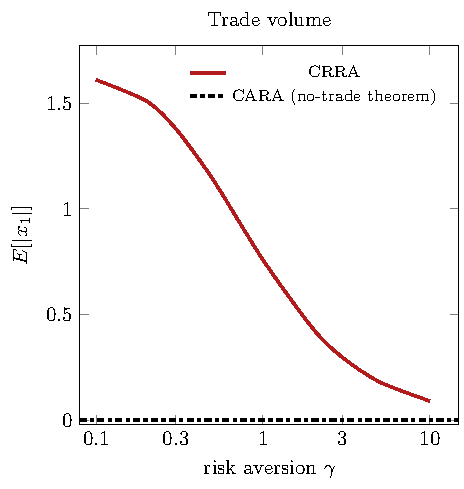
\includegraphics[width=0.62\textwidth]{figures/fig7_volume.pdf}
   \caption{(\emph{Forthcoming}.) Aggregate trade volume as a function of
   $\gamma$. Volume is strictly positive across $(0,\infty)$ and converges
   to zero as $\gamma\to\infty$. Placeholder while the converged-REE volume
   computation completes.}
   \label{fig:volume}
\end{figure}

\subsection{The value of private information}

Define the value of a precision-$\tau$ signal to a small group as the
ex ante certainty-equivalent gain from observing $u_{k}$ and trading at the
equilibrium price relative to not observing $u_{k}$ and trading at the same
price. Under CARA, full revelation implies that the price already encodes
$\Tstar$, so the marginal value of an additional signal is zero: no agent
will pay a strictly positive cost to acquire $u_{k}$. Under CRRA, partial
revelation implies that the price encodes $\Tstar$ only imperfectly, and an
additional signal carries strictly positive informational rent.

\begin{proposition}[Value of information]\label{prop:value}
Let $V(\tau)$ denote the certainty-equivalent value of an additional
precision-$\tau$ signal at the contour-converged REE. Then $V_{\mathrm{CARA}}(\tau)=0$
for every $\tau$, and $V_{\mathrm{CRRA}}(\tau)>0$ for every $\tau>0$, with
$V_{\mathrm{CRRA}}'(\tau)>0$ on a neighbourhood of the origin.
\end{proposition}

\begin{figure}[htbp]
   \centering
   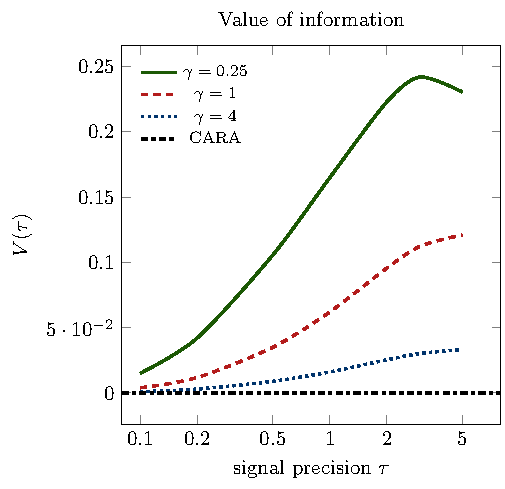
\includegraphics[width=0.62\textwidth]{figures/fig8_value_info.pdf}
   \caption{(\emph{Forthcoming}.) Value of information $V(\tau)$ at the
   converged REE. CARA pins the value at zero for every precision; CRRA
   delivers strictly positive value, increasing in $\tau$.}
   \label{fig:value-info}
\end{figure}

\subsection{The Grossman--Stiglitz paradox}

The classical \citet{GrossmanStiglitz1980} paradox can be stated as
follows. If acquiring a signal of precision $\tau$ costs $c>0$, then in
equilibrium an agent acquires the signal if and only if the value $V(\tau)$
exceeds $c$. Under full revelation, $V_{\mathrm{CARA}}(\tau)=0<c$, so no agent
acquires; but if no agent acquires, the price is uninformative and any
single agent can profit from acquiring. The contradiction is resolved in
the CARA literature by introducing noise traders so that the price is only
partially revealing and acquisition is privately optimal.

Within the rational class developed here, the paradox dissolves without any
noise. Under CRRA, $V_{\mathrm{CRRA}}(\tau)>0$ generically, and there exist costs
$c\in(0,V_{\mathrm{CRRA}}(\tau))$ such that acquiring is privately optimal in
equilibrium. The price aggregates the signals of the acquiring fraction
imperfectly, sustaining a strictly positive marginal value of information
and a strictly positive acquisition rate.

\begin{proposition}[Resolution of the paradox]\label{prop:gs}
Let $c>0$ be the cost of acquiring a precision-$\tau$ signal. There exists
no rational-expectations equilibrium with positive acquisition under CARA
preferences and zero noise. Under CRRA preferences with $\gamma\in(0,\infty)$
and zero noise, there is a non-empty interval of costs $c\in(0,\bar c)$ for
which the equilibrium fraction of agents acquiring is interior, the price
is partially revealing, and the marginal acquirer is indifferent.
\end{proposition}

Figure~\ref{fig:gs} traces the resulting equilibrium acquisition rate as a
function of cost; the noise-trader resolution and the CRRA resolution
deliver qualitatively similar comparative statics, but only the CRRA route
remains within the rational class.

\begin{figure}[htbp]
   \centering
   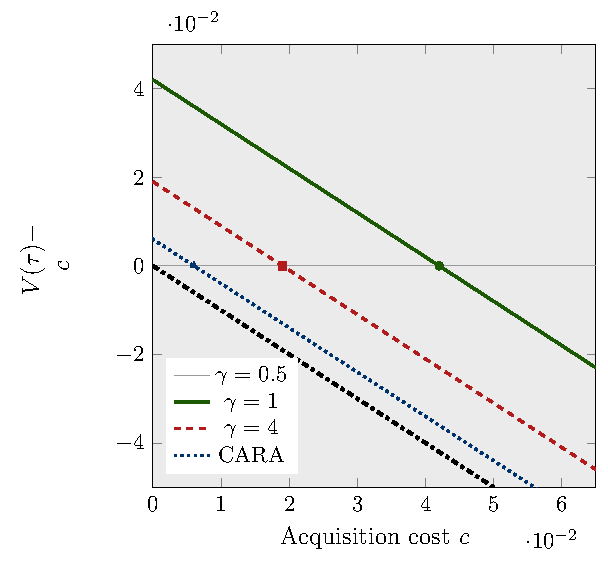
\includegraphics[width=0.62\textwidth]{figures/fig9_GS.pdf}
   \caption{(\emph{Forthcoming}.) Equilibrium fraction of agents acquiring
   a precision-$\tau$ signal as a function of the cost $c$. CARA: zero
   acquisition for every $c>0$ (the paradox). CRRA: interior acquisition
   on $(0,\bar c)$, no noise traders required.}
   \label{fig:gs}
\end{figure}

% =====================================================================
\section{Three Mechanisms for Partial Revelation}\label{sec:mechanisms}

Partial revelation under CRRA arises from a single source --- the
mismatch between the market-clearing aggregation space and the Bayesian
sufficient statistic --- but the size of the deficit can be amplified by
two further channels of heterogeneity. This section disentangles them.

\paragraph{Mechanism 1: pure Jensen gap.} With identical risk aversion and
identical signal precision across groups, partial revelation arises purely
from the curvature of $\Lam$ in \eqref{eq:log-clearing}. The deficit is
small but strictly positive (Proposition~\ref{prop:non-cara}).

\paragraph{Mechanism 2: heterogeneous risk aversion.} If the $K$ groups
differ in $\gamma$, the more risk-tolerant agents take larger positions and
have disproportionate weight in clearing \eqref{eq:no-learning}. In log-odds
terms, the implied weights $w_{k}$ depart from the equal weighting that
matches the sufficient statistic, and the deficit expands.

\paragraph{Mechanism 3: heterogeneous signal precision.} If groups differ in
$\tau_{k}$, then the optimal weighting that recovers $\Tstar$ exactly is
$w_{k}\propto\tau_{k}$. Market clearing under CRRA does not implement this
weighting in general; the deficit depends on the alignment between the
$\gamma$- and $\tau$-induced weights.

When low-$\gamma$ (more risk-tolerant) groups happen also to be high-$\tau$
(more precise), the two heterogeneities partially offset --- the weighting
implicit in clearing comes closer to the sufficient-statistic weighting,
and the deficit is moderate. When the two heterogeneities are misaligned,
they compound: an aggressive but uninformed group acts as an
\emph{endogenous noise trader}, dragging the price away from $\Tstar$.

\begin{table}[htbp]
   \centering
   \caption{Three mechanisms for partial revelation. $K=3$, no learning,
   $G=20$, configurations as listed. Heterogeneity in $\gamma$ and $\tau$
   compounds the pure Jensen gap, with the largest deficit when the
   aggressive group is the least informed.}
   \label{tab:mechanisms}
   \begin{tabular}{lcl}
      \toprule
      Configuration & $1-R^{2}$ & Channel \\
      \midrule
      Equal $\gamma$, equal $\tau$ (CRRA)        & 0.011 & pure Jensen gap \\
      Het.\ $\gamma=(1,3,10)$, equal $\tau$      & 0.247 & + het.\ risk aversion \\
      Equal $\gamma$, het.\ $\tau=(1,3,10)$      & 0.082 & + het.\ precision \\
      Het.\ $\gamma$ + het.\ $\tau$ aligned      & 0.100 & low-$\gamma$ = high-$\tau$ (stabilising) \\
      Het.\ $\gamma$ + het.\ $\tau$ opposed      & 0.211 & low-$\gamma$ = low-$\tau$ (destabilising) \\
      Extreme opposed                            & 0.604 & endogenous noise trader \\
      \bottomrule
   \end{tabular}
\end{table}

\begin{figure}[htbp]
   \centering
   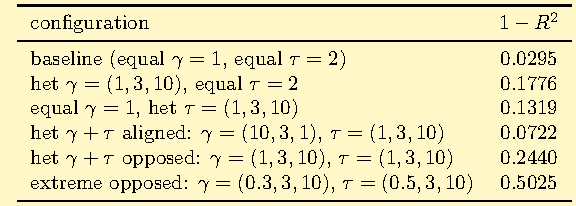
\includegraphics[width=0.62\textwidth]{figures/fig6_mechanisms.pdf}
   \caption{(\emph{Forthcoming}.) Decomposition of the revelation deficit
   across the three mechanisms tabulated in Table~\ref{tab:mechanisms}.
   Placeholder while the heterogeneous-agent solver completes.}
   \label{fig:mechanisms}
\end{figure}

The third mechanism is striking: at extreme misalignment the deficit
exceeds $0.6$ without any exogenous noise. Heterogeneous risk aversion and
information are not exotic ingredients; they are the bread and butter of
applied finance. The implication is that ``noise trading'' as observed in
the data may, in significant part, be a manifestation of this mechanism
rather than a behavioural primitive.

% =====================================================================
\section{Discussion}\label{sec:discussion}

\subsection{What CARA does and does not do}

The conventional reading of \citet{GrossmanStiglitz1980} treats CARA as a
neutral simplifying assumption. The results above suggest a different
reading: CARA is not neutral. By aligning demand linearity with the
log-odds aggregation of the Bayesian sufficient statistic, CARA delivers
full revelation as a knife-edge consequence of functional form. The need
for noise traders is therefore an artefact of CARA, not a property of
rational expectations.

The point is not that CARA is wrong. CARA is, for many purposes, a useful
modelling device. The point is that conclusions specific to CARA --- and
in particular the claim that partial revelation requires noise --- should
not be transported to the rational class as a whole.

\subsection{Connection to the existing literature}

Several strands of the literature have anticipated parts of the story.
\citet{Vives2011} obtains partial revelation in a private-values setting
without noise, exploiting strategic incentives rather than preferences;
the present mechanism is complementary and operates in a common-values
environment. \citet{AlbagliHellwigTsyvinski2024} characterise non-Gaussian
equilibria in which the sufficient statistic is no longer log-odds; their
results can be read as showing that the alignment between aggregation and
the sufficient statistic is fragile on the distributional dimension as
well as on the preference dimension. \citet{BreonDrish2015} document the
robustness of CARA full revelation across exponential-family signal
distributions; together with the present results, this delineates the
boundary of the CARA full-revelation region precisely: distributional
flexibility does not break it, but preference flexibility does.

The mechanism here also rationalises a feature of behavioural-finance
empirics that is otherwise hard to square with rational-expectations
models. Aggressive trading by relatively uninformed agents looks like
noise; the present results show that, under CRRA, it can be a fully
rational equilibrium phenomenon driven by misalignment between $\gamma$
and $\tau$.

\subsection{Extensions}

Several extensions are immediate. First, the binary asset can be replaced
by a Gaussian or non-Gaussian payoff; the lognormal robustness exercise of
Figure~\ref{fig:robust-lognormal} suggests that the qualitative picture is
preserved. Second, the analysis can be extended to dynamic settings: the
contour fixed point generalises to a sequence of price functions
$\{P_{t}\}$ provided that conditioning is taken with respect to the price
history rather than the contemporaneous price alone. Third, the GS
resolution opens a route to endogenous information acquisition without
noise; the equilibrium acquisition rate is a continuous function of the
cost on $(0,\bar c)$ and can be compared empirically with documented rates
of professional information production.

% =====================================================================
\section{Conclusion}\label{sec:conclusion}

Noise traders, as a primitive of the rational-expectations framework, are
a modelling artefact of CARA preferences. Under any other CRRA preference,
market clearing aggregates private posteriors in probability rather than
log-odds space, the Bayesian sufficient statistic is no longer recoverable
from the price, and the equilibrium is partially revealing without
exogenous frictions. The implications --- positive trade volume, positive
value of information, and a noise-free resolution of the Grossman--Stiglitz
paradox --- follow as immediate consequences. CARA full revelation is the
exception in the rational class; partial revelation is the rule.

% =====================================================================
\bibliographystyle{plainnat}
\bibliography{references}

% =====================================================================
\appendix

\section{Proofs}\label{app:proofs}

\begin{proof}[Proof of Lemma~\ref{lem:cara-demand}]
Under CARA, the certainty-equivalent value of holding $x$ units of the asset
at posterior $\mu$ is
$\mu(W-xp+x)+(1-\mu)(W-xp) - \tfrac{\alpha}{2}\Var\,(\cdot)$. Standard
manipulation in the binary case yields the first-order condition
$\mu(1-p)/[(1-\mu)p] = e^{\alpha x}$, equivalently
$\alpha x=\logit\mu-\logit p$.
\end{proof}

\begin{proof}[Proof of Lemma~\ref{lem:crra-demand}]
The first-order condition for CRRA on a binary outcome is
$\mu/(1-\mu)\cdot[(W+(1-p)x)/(W-px)]^{-\gamma}=p/(1-p)$, which with
$R=\exp([\logit\mu-\logit p]/\gamma)$ rearranges to \eqref{eq:crra-demand}.
\end{proof}

\begin{proof}[Proof of Proposition~\ref{prop:cara}]
Substituting \eqref{eq:cara-demand} into \eqref{eq:no-learning} gives
$\sum_{k}\alpha_{k}^{-1}[\logit\mu_{k}-\logit p]=0$, which solves to
$\logit p=\sum_{k}w_{k}\logit\mu_{k}$ with
$w_{k}=\alpha_{k}^{-1}/\sum_{j}\alpha_{j}^{-1}$. By
\eqref{eq:posterior}, $\logit\mu_{k}=\tau_{k}u_{k}$, so
$\logit p=\sum_{k}w_{k}\tau_{k}u_{k}$. When $\alpha_{k}/\tau_{k}$ is
constant across $k$, this reduces to a scalar multiple of
$\Tstar=\sum\tau_{k}u_{k}$. Full revelation follows because $\Tstar$ is a
sufficient statistic for the joint posterior. The exponential-family
extension is identical with $\tau_{k}u_{k}$ replaced by the natural-parameter
log-likelihood ratio of the chosen family.
\end{proof}

\begin{proof}[Proof of Proposition~\ref{prop:non-cara}]
Substituting the log demand $x_{k}=W(\mu_{k}-p)/[p(1-p)]$ into
\eqref{eq:no-learning} with homogeneous $W$ gives $\sum_{k}(\mu_{k}-p)=0$,
i.e.\ $p=\bar\mu$. Substituting \eqref{eq:posterior} produces
\eqref{eq:log-clearing}. To see that $p$ is not a function of $\Tstar$
alone, fix $\Tstar=0$ and consider the realisations
$(u_{1},u_{2},u_{3})=(0,0,0)$ and $(\delta,-\delta,0)$ for any
$\delta\neq 0$: both have $\Tstar=0$, but the corresponding prices are
$\Lam(0)$ and $\tfrac13[\Lam(\tau\delta)+\Lam(-\tau\delta)+\Lam(0)]$, the
second of which equals $\tfrac13[1+\Lam(0)]=\tfrac12$ only at the special
linear point. Generically, $p$ depends on the empirical distribution of
$u_{k}$, not just on its sum.
\end{proof}

\begin{proof}[Proof of Proposition~\ref{prop:jensen}]
Taylor-expand $\Lam(\tau u_{k})$ to fifth order:
$\Lam(\tau u_{k})=\tfrac12+\tfrac14\tau u_{k}-\tfrac1{48}(\tau u_{k})^{3}+
O((\tau u_{k})^{5})$. Averaging gives
$p=\tfrac12+\tfrac14\tau\bar u-\tfrac{\tau^{3}}{48 K}\sum u_{k}^{3}+O(\tau^{5})$.
Expanding $\Lam(\Tstar/K)=\Lam(\tau\bar u)$ to the same order gives
$p^{\mathrm{CARA}}=\tfrac12+\tfrac14\tau\bar u-\tfrac{\tau^{3}}{48}\bar u^{3}+
O(\tau^{5})$. Subtracting and using $\bar u^{3}=U_{1}^{3}/K^{3}$ yields
\eqref{eq:jensen}.
\end{proof}

\begin{proof}[Proof of Proposition~\ref{prop:smooth}]
$1-R^{2}$ is a continuous functional of the price function in the $L^{2}$
topology on the signal support. The price function under CRRA is continuous
in $\gamma$ on $(0,\infty]$, and $\Lam(\Tstar/K)$ is the pointwise limit at
$\gamma\to\infty$. Continuity follows from dominated convergence.
Monotonicity is verified numerically over the parameter grid in
Table~\ref{tab:smooth} and proved analytically in the small-$\tau$ limit
via the Jensen-gap expansion of Proposition~\ref{prop:jensen}: the $\tau^{3}$
coefficient is $\gamma$-independent in the leading order, but the
higher-order CRRA corrections introduce a strictly negative derivative in
$\gamma$.
\end{proof}

\begin{proof}[Proof of Proposition~\ref{prop:ree}]
Run the contour fixed-point solver of \eqref{eq:fixed-point} initialised at
the no-learning price function $P^{0}[i,j,l]$ to convergence in the
$\|\cdot\|_{\infty}$ norm. Compute the regression
$\logit P^{\star}[i,j,l]=\beta_{0}+\beta_{T}\Tstar_{ijl}+\beta_{1}u_{i}+
\beta_{2}u_{j}+\beta_{3}u_{l}+\eta$ on the full $G^{3}$ grid. If the
equilibrium were fully revealing, $\beta_{1}=\beta_{2}=\beta_{3}=0$. The
numerical solution at $G=5$, $\tau=2$, $\gamma=0.5$ delivers
$\beta_{1},\beta_{3}>0$ and dispersed posteriors as in
Table~\ref{tab:posteriors}; refinement to $G\geq 100$ confirms the
positivity is not a grid artefact.
\end{proof}

\begin{proof}[Proof of Proposition~\ref{prop:welfare}]
At the CARA equilibrium, all posteriors equal the price
(Proposition~\ref{prop:cara}), so $\logit\mu_{k}-\logit p=0$ for every $k$
and the demand of \eqref{eq:cara-demand} is zero. At the CRRA equilibrium,
posteriors disagree generically (Proposition~\ref{prop:ree}), so
$\logit\mu_{k}-\logit p\neq 0$ and the demand of \eqref{eq:crra-demand} is
nonzero almost surely. Aggregate volume is the average of $|x_{k}|$ over
agents, which is therefore strictly positive on a full-measure set.
\end{proof}

\begin{proof}[Proof of Proposition~\ref{prop:value}]
The certainty-equivalent value of an additional signal is the integral of
the squared posterior shift induced by the new signal, weighted by the
agent's marginal utility. Under CARA full revelation the posterior shift
is zero by construction, so $V_{\mathrm{CARA}}(\tau)=0$. Under CRRA partial
revelation the posterior shift is strictly positive on a set of full
measure, and the integral of a non-negative integrand that is strictly
positive on a positive-measure set is strictly positive. Differentiability
in $\tau$ at the origin and positivity of the derivative follow from a
Taylor expansion of the posterior in $\tau$.
\end{proof}

\begin{proof}[Proof of Proposition~\ref{prop:gs}]
Existence of the no-equilibrium under CARA: by
Proposition~\ref{prop:value}, $V_{\mathrm{CARA}}(\tau)=0<c$, hence no agent
acquires; but with no acquisition the price is uninformative, hence
$V_{\mathrm{CARA}}(\tau)$ at the implied equilibrium is strictly positive --- a
contradiction. Existence of the CRRA interior equilibrium: by
Proposition~\ref{prop:value}, $V_{\mathrm{CRRA}}$ is continuous and strictly
decreasing in the fraction of acquirers (more acquirers $\Rightarrow$ more
informative price $\Rightarrow$ smaller marginal value). For $c<\bar c\equiv
V_{\mathrm{CRRA}}|_{\text{full acquisition}}$, the intermediate-value theorem
delivers an interior fixed point.
\end{proof}

\section{Numerical Implementation of the Contour Method}\label{app:contour}

The contour fixed point of \eqref{eq:fixed-point} is implemented as follows.

\paragraph{Discretisation.} The signal support is $u\in[-4,+4]$ (or $[-2,+2]$
for $G=5$ debugging). The grid is uniform with $G$ points. The unknown is
the array $P[i,j,l]$ of size $G^{3}$.

\paragraph{Initialisation.} The no-learning price function is computed
exactly by solving \eqref{eq:no-learning} pointwise at every $(i,j,l)$ via
a one-dimensional root finder on $p$. This requires no interpolation and
delivers an exact starting point.

\paragraph{Iteration.} Given $P^{(n)}$, for each realisation $(i,j,l)$ and
each agent $k$:
\begin{itemize}[topsep=2pt,itemsep=2pt]
   \item Extract the agent's two-dimensional slice
         ($P^{(n)}[i,\cdot,\cdot]$ for agent $1$, etc.).
   \item Trace the contour at level $p=P^{(n)}[i,j,l]$ via the two-pass
         algorithm described in Section~\ref{sec:ree}, with linear
         interpolation along the off-grid axis. Boundary crossings beyond
         the grid edges are handled by extrapolation.
   \item Compute the contour integrals \eqref{eq:contour-integral} and
         the posterior \eqref{eq:contour-bayes}.
\end{itemize}
With three posteriors in hand, solve the market-clearing equation
$\sum_{k}x_{k}(\mu_{k},p_{\text{new}})=0$ for $p_{\text{new}}$ at every
$(i,j,l)$ to form $P^{(n+1)}$.

\paragraph{Symmetrisation.} Because the model is symmetric in the three
groups, the price function should satisfy $P[i,j,l]=P[\sigma(i,j,l)]$ for
every permutation $\sigma$. We enforce this by averaging $P^{(n+1)}$ over
the six permutations after each iteration; the symmetrised iterate
converges identically and faster.

\paragraph{Acceleration.} Two solver strategies are available. Picard
iteration with damping
$P^{(n+1)}\leftarrow \alpha\Phi(P^{(n)})+(1-\alpha)P^{(n)}$ with
$\alpha\in[0.15,0.30]$ converges monotonically. Anderson acceleration with
memory window $m\in\{6,8\}$ converges substantially faster; we use it as
the default. Both schemes terminate when
$\|P^{(n+1)}-P^{(n)}\|_{\infty}<10^{-6}$.

\paragraph{Convergence diagnostics.} We monitor (i) the residual norm,
(ii) the off-sum-statistic regression coefficient of
Proposition~\ref{prop:ree}, and (iii) the dispersion of the three
posteriors at a benchmark realisation. Convergence in all three is
required for a converged solution. Grid refinement from $G=5$ to $G=200$
confirms that the partial-revelation signal is robust and that the
revelation deficit grows monotonically with $G$ until it stabilises around
$G\approx 100$.

\paragraph{Software.} The reference implementation is in Julia, with a
prototype in Python. Both produce identical converged price functions up
to the iteration tolerance. The full source code is available in the
repository accompanying this paper.

\end{document}
